%!TEX root = finalReport.tex
%!TEX encoding = UTF-8 Unicode
%==============================================================================

Designing hexapod legged robots is far from trivial. A very numerous and a wide range of
possibilities exist to design a hexapod as also described in the previous section. Designers must take several decisions which influence the operation and technical features. Some of the most important design issues and constraints according to \cite{48h} can be outlined as:
\begin{itemize}
	\item The mechanical structure of robot body.
	\item Leg architecture.
	\item Max sizes.
	\item Actuators and drive mechanisms.
	\item Control architecture.
	\item Power supply.
	\item Walking gaits and speed.
	\item Obstacle avoidance capability.
	\item Payload.
	\item Autonomy.
	\item Operation features.
	\item Cost.
\end{itemize}
The above mentioned design issues and constraints can be classified as design input (or key	features) and design output (or main design characteristics) as shown in the scheme of Fig.\ref{GD}.
\begin{figure}[h]		
	\centering
	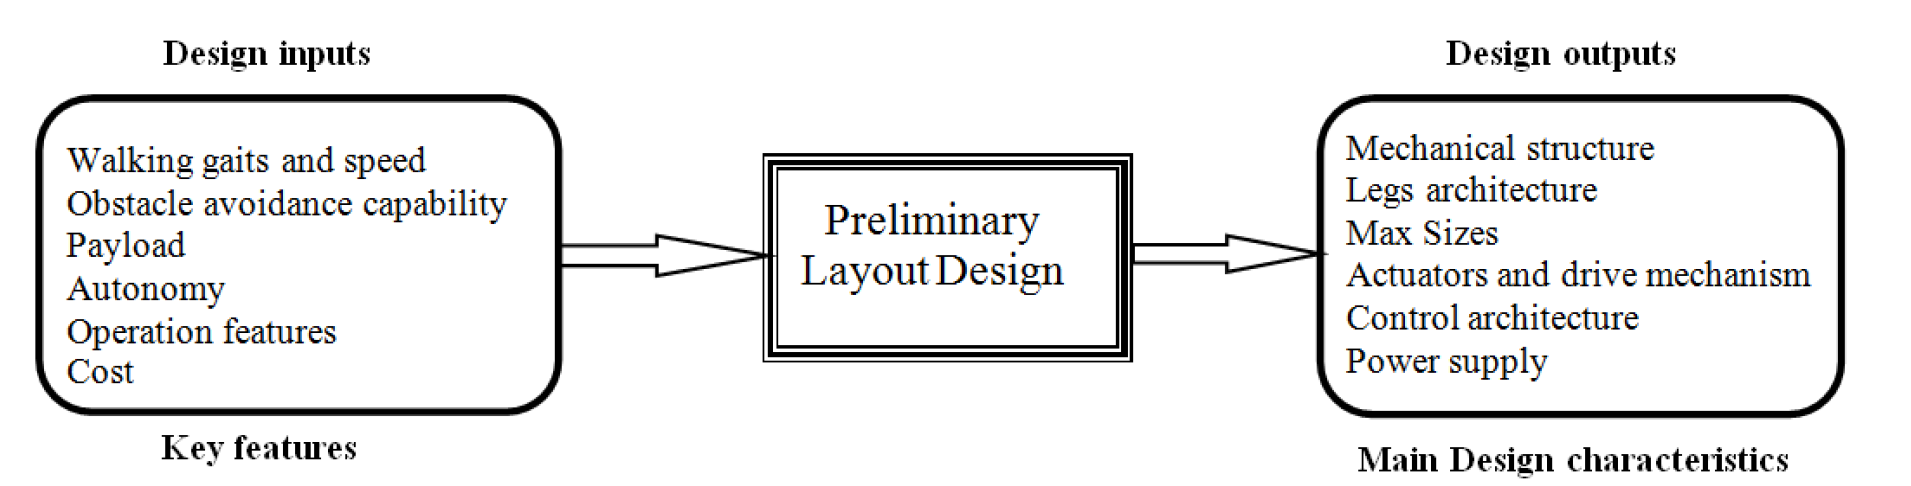
\includegraphics[width =.8\textwidth]{GD}
    \caption{ A scheme for preliminary layout design of hexapod walking robots.}
	\label{GD}
\end{figure}

\section{Hardware}
ZagHexa is a hexapod robot with 18 DOFs (three degrees of freedom (DOF) for each leg), it can walk in any direction (translation), or turn in place (rotation), or any combination of the two. The leg lift and ride height is adjustable as well. The robot uses a distributed walking control system based on the neurobiology of insects, stepping in the sagittal plane to angled stepping, which then induces turning in the robot.
It is an integrated multi-legged walking robot based on de-facto standard Robotic Operating System (ROS) that employs novel and different walking patterns.
Our robot is teleoperated using hand-held devices such as a smart phone or tablet or a wireless joystick (see Fig.\ref{fig4}). Furthermore, it has its own navigation system and a camera for instant video recording and streaming.
The power to the entire system is supplied through two 5 volts NiMH batteries. There is an additional power bank to power up the Raspberry Pi and other electronic components. 
We have an interactive website for robot inspection and online control in addition to leaning materials such as robot building and implementation walkthroughs and as well as step-by-setup tutorials.

\begin{figure}[h]
	\centering
	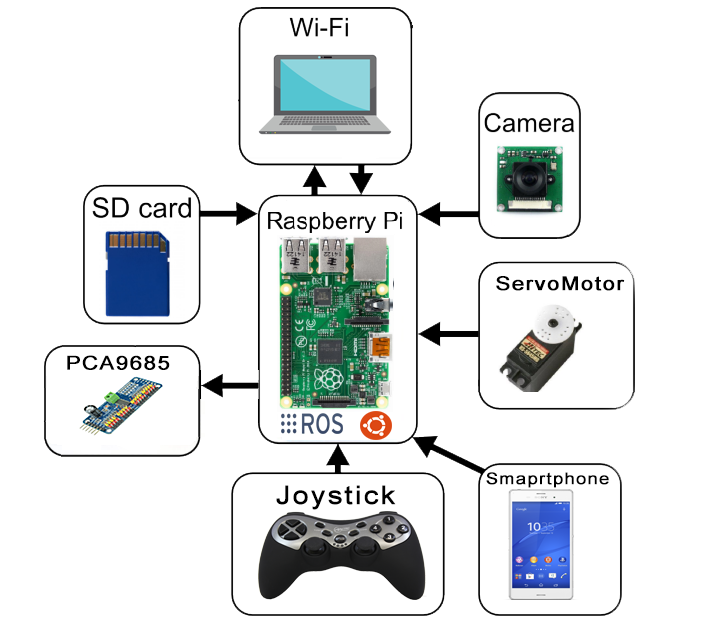
\includegraphics[width =.5\textwidth]{Fig2}
	\caption{ The electronic system of the robot.}
	\label{fig4}
\end{figure}
\subsection{Components needed}

\begin{center}
    \begin{tabular}{ |c| }
        \hline
        Metal sheet Aluminum structure         \\ \hline
        Raspberry Pi 3 Model B                       \\ \hline
        Arduino Mega                                     \\ \hline
        Metal Gear Servo motor standard size (13 kg.cm)  \\ \hline
        Metal Gear Servo motor standard size (7.5 kg.cm) \\ \hline
        Metal Servo gear hub                                             \\ \hline
        NiMH rechargeable battery (5V -1500 mAh)           \\ \hline
        Copper Spacers                                 \\ \hline
        Plastic Spacers                                  \\ \hline
        Screws and nuts                                \\ \hline
        Jumper wires                                     \\ \hline
        Power Bank 8000 mAh                       \\ \hline
        android smart phone.                         \\ \hline
    \end{tabular}
\end{center}
\section{Hardware and Software Architecture}
The final design of the ZagHexa robot constructed mainly with acrylic is shown in Fig.\ref{fig1}. ZagHexa body moves independently of its ground contact points. To make its center of gravity shift on a horizontal plane, forward/backward, and sideways moving functions are effective. These functions can also produce a smooth body movement independently of intermittent leg traveling. The robot has been designed with three degrees of freedom in the front, middle and rear legs respectively. The physical specifications are given in Table 2.\\
\begin{center}
\begin{tabular}{|c|c|}
    \hline
    Parameter       &       Description        \\ \hline
    Length         &           30cm           \\ \hline
    Width         &           27cm           \\ \hline
    Height         &           17cm           \\ \hline
    Weight         &           3Kg            \\ \hline
    Construction Material &                          \\ \hline
    Actuators       &     DC servo motors      \\ \hline
    Motion Control     & Servo Sequential Control \\ \hline
    Leg Stroke (Max)    &           6cm            \\ \hline
    Leg Lift (Max)     &           5cm            \\ \hline
\end{tabular}
\end{center}

\subsection{Hardware Architecture}
As illustrated in Fig.\ref{fig4}, ZagHexa is equipped with all necessary resources to interact with the environment. The system is supplied with an embedded computing system, which is Raspberry Pi 3 Model B running Ubuntu Xilinx. \\
Raspberry Pi is a miniature computer the size of a credit card, to which a standard monitor, a keyboard and a mouse can be connected.\\
It has extremely low power consumption (max. 3.5 W) and can run ROS based on Ubuntu operating system. There are several models, which differ in RAM, the number of USB ports or GPIO pins and the connation methods. Raspberry Pi is equipped with a USB Wi-Fi dongle, which is connected to a wireless network, and runs Qt [11] client program, that connects to the server and communicate with it. Sensor data are sent to a computer after successful connection. Client is also capable of automatically reconnect in case of connection disruption.\\
To sense the environment and deal with it, different modalities of sensors are imported from an attached smart hand-held device. As ZagHexa can use all the sensors form any mobile phone thanks to its own android subsystem that communicate these information with the smart phone over Wi-Fi or Bluetooth.\\
\subsection{Joint Actuators}
The leg joints are actuated by metal gear servos: FS5113M on coxa, femur and FS5106M on tibia joints. These motors were chosen for their high torque. Each of the three joint actuators per leg directly drives its associated leg segment. By attaching the leg segment directly to the servo output horns, the mechanical design of the joints is simplified.  This direct connection also allows the joints to take advantage of the nominal $\pm90deg$ range-of motion (RoM) of the servos, which is approximately the same RoM as the insect  \cite{17}.

It is important for the leg control system to know current joint angles (servo position) and joint loads (current consumption). As this information is not available from standard servos, the motors were modified. The servo internal PCB, which is responsible for receiving PWM position commands from a host   and   converting   those   commands   into   servo   output positions.
All servomotors are connected and driven by the PCA9685 controller. This controller receives the desired walking pattern from the Raspberry through I2C pins controlling the leg lift-swing-shift sequence.

\section{Software}
The high–level functionality and control of the robot are implemented in ROS packages. The Robot Operating System (ROS) is a standard and open–source operating system for robot control \cite{9}. ROS is not an operating system in the traditional sense of process management and scheduling; rather, it provides a structured communication layer above the host operating systems of a heterogeneous compute cluster. Our software ROS packages interact with each of the subsystems in C++ and Python for direct system control. The system described uses a Linux based software framework as an operating system (OS) for providing the advantages of using an OS, which supports developing additional modules that can be easily implemented and integrated. 

ROS provides operating system like service for the robot. It is a meta-operating system, which loads on top of an operating system to provide a standardized set of software framework and APIs. These facilities cannot only help robots but also other embedded systems with a rich set of tools to successfully manage the complexity. With ROS handling the basic communications and data exchange.